\section{Diagrammes de classes}
La modélisation de tout système passe essentiellement par un diagramme de classes qui
englobe les différentes entités et les relations entre elles. Compte tenu des spécifications établies dans
les chapitres précédents, le diagramme de classes global du système contient un certain nombre de
classes : 
\begin{itemize}[label=\textbullet]
\item Pays : entité qui représente une aire géographique dans laquelle se trouve les clients 
\item Région : entité qui rassemble les pays
\item Agence : entité qui rassemble les régions
\item Client : entité qui représente les clients de l'entreprise
\item Ressource : entité qui représente les employés de l'entreprise 
\item RessourceAdmin : entité qui représente les ressources qui travaille au sein de la direction de l'entreprise
\item RessourceProjet : entité qui représente les ressources qui implémente le produit chez le client 
\item Profil : entité qui représente le poste que les ressources occupent
\item SuiviFDT : entité représente le nombre de FDT manquantes par semaine pour chaque ressource
\item AffectationClient : entité qui représente la liste des directeurs de projet de chaque client
\item AffectationRessource : entité qui représente la liste des supérieurs et profils de chaque ressource projet 
\item RemplacementRessource :  entité qui représente le remplacement d'une ressource projet par une autre
\item Rubrique : entité qui représente une rubrique dans laquelle une ressource sera évaluée
\item Module : entité qui rassemble des rubriques
\item Domaine : entité qui rassemble des modules
\item NiveauCompetence : entité contenant les informations sur un niveau de compétence
\item Evaluation : entité qui rassemble l'ensemble des évaluations des ressources
\end{itemize}
\newpage
\begin{figure}[h!]
 \centering
     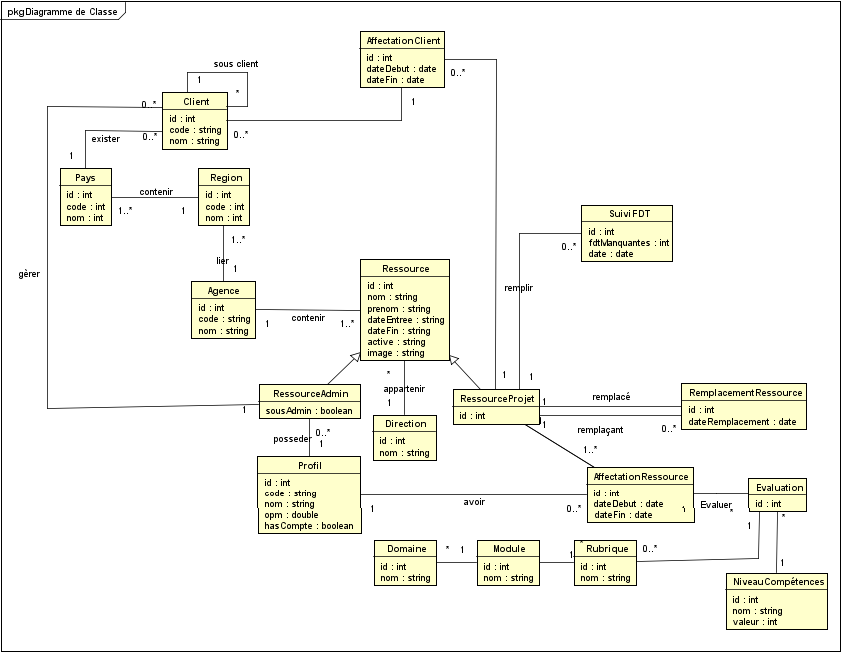
\includegraphics[width=1.4\textwidth,angle=90]{chapitre4/Figures/classes.png}
\caption{Diagramme de classes principal}
\end{figure}%sidewaysfigure
\newpage
\begin{figure}[h!]  
 \centering
    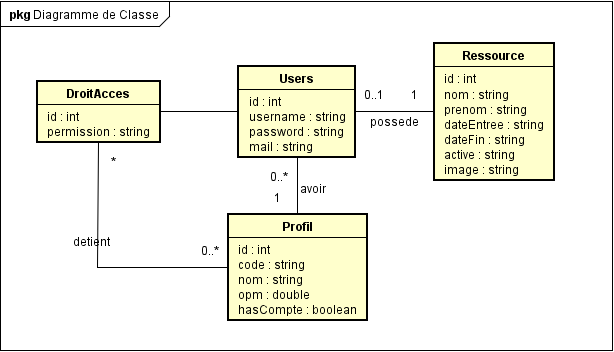
\includegraphics{chapitre4/Figures/cnx.png}
  \caption{Diagramme de classes élémentaire (Gestion des droits d’accès)}
\end{figure}

Chaque utilisateur a un rôle. Les utilisateurs ayant le même rôle ont les mêmes droits d'accès. Un rôle peut-être acquis par plusieurs ressources.